% =====================================================================
\chapter{A \Mimir{} rendszer jelenlegi állapota és generálási módszere}
\label{ch:modszer}
\chaptermark{A \Mimir{} rendszer}
% =====================================================================

Ebből a fejezetből az olvasó megtudja, hogyan épül fel ma a \Mimir{}, hogyan kezeli a tananyagot, és
hogyan felel meg az adatvédelmi és az MI-rendeleti követelményeknek
(\ref{sec:architektura}--\ref{sec:megfeleles}.~szakasz); mekkora GPU-memóriát igényel a helyi futtatás
(\ref{sec:vram}.~szakasz); végül lépésenként megismeri a vizsgált generálási módszert
(\ref{sec:attekintes}.~szakasz). A \Mimir{} fejlesztési fázisban lévő rendszer: az éles szolgáltatások ma
a naiv RAG-ot (\arm{E0}) futtatják, a tervezett folyamat -- vizsgaterv, kérdéshelyenkénti keresés,
ellenőrző lánc, kérdésenkénti forráshivatkozás -- a kiértékelő keretrendszerben készült el
(\code{tests/new eval/mimir\_eval/blueprint}), és hogy mely elemei kerülnek be, azt
\az{\ref{ch:diszkusszio}}.~fejezet mérésen alapuló döntése határozza meg. A fejezet a szolgáltatások mai
működését a forráskód, a módszert a keretrendszer implementációja alapján írja le; a részleteket
\az{\ref{app-modszer}}.~függelék, a paramétereket \az{\ref{app-reprodukcio}}.~függelék tartalmazza.

% ---------------------------------------------------------------------
\section{Tervezési célok}
\label{sec:architektura}
% ---------------------------------------------------------------------

A bevezetés P1--P4 problémáiból és az MI-rendelet emberi felügyeletre vonatkozó elvárásából~\cite{aiact2024}
öt tervezési célt vezettünk le (\ref{tab:celok}.~táblázat). A táblázat a célállapotot írja le: a G3 és a
G5 elemei az éles rendszerben is működnek, a G1 és a G2 ma csak a kiértékelő keretrendszerben.

\begin{table}[htbp]
\centering
\caption[Tervezési célok: a csevegő nyelvi modell és a \Mimir{} összevetése.]{Tervezési célok: a
dokumentum csevegő nyelvi modellnek való átadása és a \Mimir{} célállapota.}
\label{tab:celok}
\small
\begin{tabularx}{\textwidth}{@{}>{\raggedright\arraybackslash}p{2.6cm}>{\raggedright\arraybackslash}X>{\raggedright\arraybackslash}X@{}}
\toprule
Cél & Dokumentum $\to$ csevegő modell & \Mimir{} (célállapot) \\
\midrule
G1 Ellenőrizhető & A kulcs nincs ellenőrizve, nincs forráshivatkozás & Minden kérdés a forrásrészletekre hivatkozik; alátámasztottsági és vak megoldási ellenőrzés; az ellenőrzésen át nem jutott kérdés megjelölve \\
G2 Kontrollált & Darabszám, típus, nehézség csak kérés & A vizsgaterv rögzíti a darabszámot, a típusokat és a Bloom-szinteket; lefedettségvezérelt fogalomválasztás \\
G3 Adatvédő & Az anyag a szolgáltatóhoz kerül & Választható helyi modell; a feldolgozási adatok a feladat végén törlődnek; kapcsolható, kizárólag helyi mód \\
G4 Megvalósítható & Hosszú kontextus, nagy modell & Rövid hívások 8\,192 tokenes kontextusban; fogyasztói GPU (8--12\,GiB) \\
G5 Felügyelt & A kimenet változtatás nélkül használható & Kötelező oktatói jóváhagyás szerkesztőben, a hivatkozott forrással; MI-közreműködés jelölése az exportban \\
\bottomrule
\end{tabularx}
\end{table}

% ---------------------------------------------------------------------
\section{Architektúra és megvalósítás}
\label{sec:megvalositas}
% ---------------------------------------------------------------------

A rendszer konténerizált, verziózott (\code{/api/v1}) felületű FastAPI-szolgáltatásokból áll, amelyeket
egy nginx-alapú API-átjáró fog össze (\ref{fig:architektura}.~ábra); nevüket az északi mitológia
tudással kapcsolatos alakjairól kapták:
a \emph{Wellspring} PDF-ből, DOCX-ből és szövegfájlból nyeri ki a szöveget (olvashatatlan oldalnál a
GenAI-szerver képfelismerő modelljével, ennek hiányában vagy helyi módban Tesseract OCR-rel);
a \emph{RuneCarver} mondatokra bont, beágyaz és darabol (\ref{sec:darabolas}.~szakasz);
a \emph{Bifrost} indexel, keres, promptot épít, modellt választ és a generálási feladatokat kezeli;
a \emph{Heimdall} a kész vizsgát egy nyelvi modellel 1--10-es koherencia-pontszámmal értékeli, ez az
audit naplóba kerül, de a kimenetet nem szűri;
a \emph{The Forge} az audit naplót és egy adatbázis-alapú feladatsort kezel;
a \emph{Skald} JSON, Moodle XML és PDF formátumba exportál, és kérésre elmenti a jóváhagyott vizsgát.
A dokumentumfeldolgozás, a darabolás, a RAG-folyamat, a feladatkezelés és az export (Moodle XML
CDATA-blokkokkal és MathJax-támogatással, PDF saját tördelőkóddal) saját implementáció. A kiértékelő
keretrendszer az előkészítéshez ugyanezeket a végpontokat hívja, a generálást viszont a saját kódjában
futtatja (\ref{sec:harness}.~szakasz).

\begin{figure}[htbp]
\centering
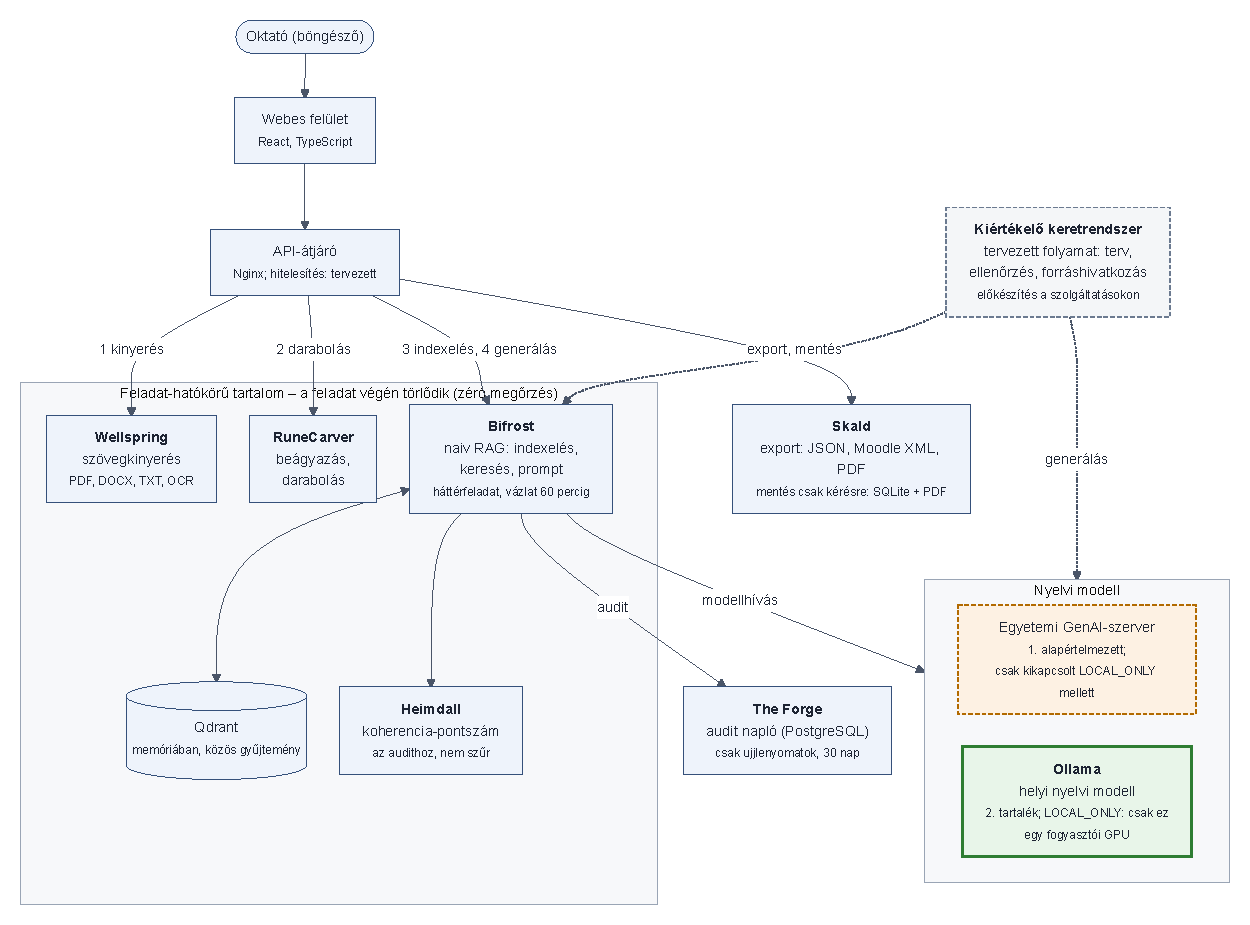
\includegraphics[width=\textwidth]{figures/d1_architektura}
\caption[A \Mimir{} szolgáltatásai és adatfolyama.]{A \Mimir{} szolgáltatásai és adatfolyama. A feltöltött
tartalmat a feldolgozó szolgáltatások csak a feladat élettartama alatt, memóriában tartják; a beágyazó
modellek CPU-n futnak, a GPU-t csak a helyi nyelvi modell használja. Külső modellt a rendszer csak
kikapcsolt \code{LOCAL\_ONLY} kapcsoló mellett hív. A számok a webes felület hívási sorrendjét jelölik; a
szürke, szaggatott keretes blokk a kiértékelő keretrendszer, amelyben a tervezett folyamat fut.}
\label{fig:architektura}
\end{figure}

\paragraph{Az éles generálási útvonal.} A webes felület a szolgáltatásokat az átjárón át, egymás után
hívja: kinyerés, darabolás, indexelés, generálás, állapotlekérdezés. A \code{/api/v1/generate} végpont
azonnal feladatazonosítót ad vissza, a generálást a FastAPI \code{BackgroundTasks} mechanizmusával, a
Bifrost folyamatában indítja; az állapot (szakasz, haladás, becsült hátralévő idő) a
\code{/api/v1/status} végponton kérdezhető le. A memóriabeli feladattár a feladatot és eredményét az
indítás után 3\,600\,s-mal (\code{JOB\_TTL\_SECONDS}) eldobja. A modellt a Bifrost alapból az egyetemi
GenAI-szerverről kéri (sorrendben \code{gpt-oss:120b}, \code{Qwen3.8-Flash-Next}); ha ez nem ad
értelmezhető választ, vagy nincs API-kulcs, a helyi Ollamára vált (alapból PULI-LlumiX 8B, Q4\_K\_M,
16\,384 tokenes kontextus, $T=0$), és ha az is hibázik, rögzített hibaüzenet-vizsgát ad vissza;
bekapcsolt \code{LOCAL\_ONLY} mellett csak a helyi modellt hívja. A feladat végén -- sikertől
függetlenül -- a \code{\_purge\_document\_data} függvény kiüríti a vektortárat.

\paragraph{Feladatsor és egyidejű használat.} A The Forge PostgreSQL-alapú feladatsora a
\code{FOR UPDATE SKIP LOCKED} záradékra~\cite{postgres2024skiplocked} épül: a munkás a legrégebbi, még
nem zárolt feladatot veszi ki, így egy feladatot pontosan egy munkás kap meg, üzenetközvetítő nélkül. A
sor ma egyetlen feladattípust ismer (darabok indexelése), és a webes folyamat nem használja. A Bifrost
vektortára memóriában futó Qdrant~\cite{qdrant2024} \emph{egyetlen közös gyűjteménnyel}, amelyet minden
indexelés és minden feladat vége kiürít. Ez egy felhasználónál a zéró megőrzést szolgálja, egyidejű
felhasználóknál viszont a dokumentumok összekeveredhetnek, vagy egy új indexelés törölheti egy futó
feladat darabjait: az éles rendszer ma egyfelhasználós, egydokumentumos üzemre alkalmas.

\paragraph{A webes felület.} A React és TypeScript alapú, kétnyelvű felületen az oktató feltölti a
dokumentumot, megadja a kérdések számát, típusát (feleletválasztós, igaz-hamis, kifejtős) és nehézségét, majd a vázlatot a szerkesztőben
(\ref{sec:felugyelet}.~szakasz) átnézi és exportálja. A \emph{legacy} API-mód a mai backendet hívja, és
éles buildben ez az alapértelmezett; a \emph{v1} mód a témakör-munkaterületet valósítja meg egy új
API-szerződésen (témakörök, fájlok, feladatok, kérdésenkénti forráshivatkozás). Ezt a szerződést a mai
szolgáltatások még nem valósítják meg, ezért a v1 felület fejlesztéskor böngészőben futó ál-backenddel
(MSW) működik; a tervezett folyamat élesítése a v1 szerződés szerveroldali megvalósítását is jelenti.

% ---------------------------------------------------------------------
\section{Adatvédelem: zéró megőrzés a feldolgozási adatokra}
\label{sec:zero}
% ---------------------------------------------------------------------

A G3 cél az adattakarékosság és a korlátozott tárolhatóság GDPR-elvén~\cite{gdpr2016} alapul. A projekt
ezt „zéró megőrzésnek” nevezi, pontosabban: a feltöltött tartalom és minden belőle számolt adat (darabok,
beágyazások, prompt) csak a feladat végéig él, a generált vázlat legfeljebb 60 percig marad a szerveren, a
jóváhagyott vizsgát pedig a Skald csak kifejezett kérésre, beállítható ideig (alapból 365 napig) tárolja.
Az adatfajták részletes életciklusát \az{\ref{tab:eletciklus}}.~táblázat
(\ref{app-eletciklus}.~függelék) foglalja össze.

Az audit napló az elszámoltathatóság miatt fontos, de nem tartalmazhat tananyagot: a feladat azonosítóját,
a modell nevét, a promptverziót és a Heimdall pontszámát tárolja, a kérésből, a promptból és a
kontextusból pedig csak a SHA-256 \emph{ujjlenyomatot} (kriptográfiai kivonatot) és a szöveg hosszát, 30
napig. Az ujjlenyomattal igazolható, hogy két futás ugyanazzal a kontextussal dolgozott-e, a tartalom
azonban nem állítható vissza belőle; a korábbi, szöveget is tároló oszlopokat a The Forge induláskor
kiüríti. A \code{LOCAL\_ONLY} kapcsoló a Bifrostban, a Heimdallban és a Wellspringben minden külső
modellhívást letilt. Alapértéke kikapcsolt, vagyis a mai telepítés a visszakeresett darabokat az egyetemi
szervermodellnek küldi; a felület minden feltöltés előtt jelzi, hol történik a feldolgozás.

% ---------------------------------------------------------------------
\section{Adatvédelem és MI-rendelet a megvalósításban}
\label{sec:megfeleles}
% ---------------------------------------------------------------------

A jogi keretet~\cite{gdpr2016,aiact2024} \az{\ref{sec:irod-jog}}.~szakasz mutatja be; itt azt foglaljuk
össze, hogyan jelennek meg a követelmények a kódban és az üzemeltetési dokumentációban. A projekt
megfelelőségi dokumentációja (\code{docs/gdpr/compliance.hu.md}, 2026.~szeptemberi tervezet) minden elemet
\emph{Megvalósítva}, \emph{Részben megvalósítva} vagy \emph{Tervezett} jelöléssel lát el;
\az{\ref{tab:megfeleles}}.~táblázat ezeket változtatás nélkül veszi át. A dokumentáció mérnöki tervezet,
nem jogi vélemény: éles indulás előtt adatvédelmi tisztviselőnek vagy jogásznak kell átnéznie, és több
adatkezelői adata (az adatkezelő neve, a tárhelyszolgáltató, az incidensfelelős) még kitöltetlen.

\begin{table}[htbp]
\centering
\caption[Adatvédelmi és MI-rendeleti követelmények és megvalósításuk.]{Adatvédelmi és MI-rendeleti
követelmények és megvalósításuk a \Mimir{} rendszerben. Az állapot a megfelelőségi dokumentáció
(\code{docs/gdpr/compliance.hu.md}) jelölése.}
\label{tab:megfeleles}
\small
\begin{tabularx}{\textwidth}{@{}>{\raggedright\arraybackslash}p{3.5cm}>{\raggedright\arraybackslash}X>{\raggedright\arraybackslash}p{2.9cm}@{}}
\toprule
Követelmény & Megoldás a rendszerben & Állapot \\
\midrule
GDPR 5.~cikk (1) c), e): adattakarékosság, korlátozott tárolhatóság & A feldolgozási adatok törlése minden feladat után; a feladat eredménye 60 perc után lejár & Megvalósítva \\
GDPR 25.~cikk: alapértelmezett adatvédelem & A vizsga mentése csak kérésre, a megőrzési idő jelzésével; mentett vizsga legfeljebb 12 hónapig & Megvalósítva \\
GDPR 5.~cikk (2); MI-rendelet: naplózás & Csak metaadatot és ujjlenyomatot tartalmazó működési napló, 30 napos megőrzés, a régi adatok kiürítése & Megvalósítva \\
GDPR 28., 44--49.~cikk: adatfeldolgozó, továbbítás & Helyi mód (\code{LOCAL\_ONLY}): nincs hívás az egyetemi GenAI-szerver felé & Megvalósítva (alapból kikapcsolva) \\
 & Adatfeldolgozói szerződések (tárhely, egyetem, e-mail) & Tervezett \\
GDPR 12--13.~cikk: tájékoztatás & Adatkezelési tájékoztató magyarul és angolul; figyelmeztetés és megerősítés feltöltéskor; a feldolgozás helye minden feltöltés előtt látható & Megvalósítva (a tájékoztató kitöltendő mezőkkel) \\
GDPR 15--20.~cikk: érintetti jogok & Mentett vizsga törlése; „Adataim” oldal a böngészőben tárolt adatokhoz & Megvalósítva (a törlés \code{user\_id} alapú tulajdonos-ellenőrzéssel) \\
 & Fiókexport és -törlés & Tervezett \\
GDPR 32.~cikk: biztonság & Hozzáférési napló paraméterek nélkül, rövidített IP-címmel & Megvalósítva \\
 & Naplórotáció: méretalapú rotáció kész, a 14 napos időkorlát üzemeltetési feladat & Részben megvalósítva \\
 & Valódi hitelesítés és tulajdonos-ellenőrzés & Tervezett \\
 & Vektoradatok elkülönítése (témakörönként) & Tervezett \\
GDPR 35.~cikk: hatásvizsgálat & Előszűrés elkészült; teljes hatásvizsgálat a bevezetés előtt & Tervezett \\
MI-rendelet 50.~cikk: átláthatóság & Figyelmeztetés a felületen; a tájékoztató MI-ről szóló pontja; a PDF metaadat-oldala jelzi az MI közreműködését és a modellt; a szerkesztő kiírja a modellt & Megvalósítva \\
MI-rendelet: emberi felügyelet (vö.\ 14.~cikk) & Kötelező ellenőrzési lépés a szerkesztőben az export előtt & Megvalósítva \\
\bottomrule
\end{tabularx}
\end{table}

\paragraph{MI-rendeleti besorolás.} Az MI-rendelet III.~mellékletének 3.~pontja az oktatásban a tanulási
eredmények értékelésére és a tanulási folyamat irányítására használt rendszereket magas kockázatúnak
minősíti. A dokumentáció értelmezése szerint a \Mimir{} mai feladata, a tanár által teljes egészében
ellenőrzött kérdések \emph{generálása}, ezen kívül esik: a rendszer nem értékel és nem pontoz vizsgázókat,
és nem hoz a GDPR 22.~cikke szerinti automatizált döntést. A diákválaszok automatikus pontozása viszont a
magas kockázatú kategóriába sorolná, ezért pontozási funkció csak új értékelés után vezethető be. A
kötelező oktatói jóváhagyás (G5) így a besorolás egyik érve is.

\paragraph{Nyitott pontok.} A bevezetés előtt három hiányt kell megszüntetni: a valódi hitelesítést (a
mentett vizsgák végpontjai ma egy \code{user\_id} paraméterben bíznak meg; a dokumentáció szerint ez a
legmagasabb prioritás), a közös vektortár témakörönkénti elkülönítését (a feladat utáni törlés a
kockázatot csak részben csökkenti) és az egyetemi GenAI-szerverrel kötendő írásos adatfeldolgozói
megállapodást; addig csak a \code{LOCAL\_ONLY} mód garantálja, hogy a szöveg nem hagyja el az üzemeltető
szerverét. Az MI-jártasságra (4.~cikk) vonatkozó teendőket a dokumentáció nem tárgyalja. A tervezett
témakör-munkaterület a darabokat és a beágyazásokat témakörönként, titkosítva megőrizné (javaslat: 90 nap
inaktivitásig), ami a zéró megőrzést módosítaná; kiadás előtt a dokumentációt és a tájékoztatót is
frissíteni kell.

% ---------------------------------------------------------------------
\section{A GPU-memória becslése}
\label{sec:vram}
% ---------------------------------------------------------------------

A G4 cél kvantitatív kérdés: elfér-e a generátor egy fogyasztói videokártyán az asztali környezet
mellett? A memóriát bináris egységekben adjuk meg ($1\ \text{GiB}=2^{30}$ bájt), mert a GPU-memória és
az Ollama által jelzett foglalás is így értendő; a kereskedelemben „8 GB-os” és „12 GB-os” kártyák
memóriája 8, illetve 12\,GiB. Az igény a kvantált súlyok, a kontextussal arányos KV-gyorsítótár és a
futtatókörnyezet többletének összege; a képletet, a Qwen2.5-7B-re végzett levezetést és öt modell
becslését \az{\ref{eq:vram}}.~egyenlet és \az{\ref{tab:budget}}.~táblázat (\ref{app-vram}.~függelék)
tartalmazza. A Q4\_K\_M kvantálás kb.\ 4,8 bit/súllyal a súlyokat a 16 bites méret nagyjából harmadára
csökkenti. A becslés szerint 8\,192 tokenes kontextusnál a Qwen2.5-7B kb.\ 5,4\,GiB-ot, a
Llama-3.1-8B-vel azonos architektúrájú PULI-LlumiX 8B kb.\ 6,1\,GiB-ot igényel, a Gemma 3 12B mért
foglalása kb.\ 7,8\,GiB (rétegeinek többsége csak egy rövid ablakra figyel, ezért a képlet nála
túlbecsül). A következtetés két fogyasztói szint: a 7--8B modellek 4 bites kvantálással elférnek egy
8\,GiB-os kártyán, a 12B modell az asztali környezettel együtt 12\,GiB-os kártyát igényel. A kontextus
növelése sem ingyenes (32\,768 tokennél a Qwen2.5-7B gyorsítótára önmagában 1,75\,GiB), ezért a helyi
teljes dokumentumos alapvonal 16\,384 tokennel és 30\,000 karakterre csonkolt dokumentummal fut, a
tervezett folyamat hívásai viszont rövidek. A mért értékeket \az{\ref{sec:fo-eroforras}}.~szakasz közli.

% ---------------------------------------------------------------------
\section{A generálási módszer}
\label{sec:attekintes}
% ---------------------------------------------------------------------

\Az{\ref{fig:pipelines}}.~ábra a két összehasonlított generálási folyamatot mutatja. A \emph{naiv RAG}
(\arm{E0}, a mai éles útvonal) a felhasználói kéréshez leginkább hasonló három darabot keresi vissza, és
egyetlen hívásban kéri a teljes vizsgát; ez a legolcsóbb ésszerű alapvonal. A \emph{tervezett folyamat}
(\arm{E1}--\arm{E3}) először explicit vizsgatervet készít, majd a terv minden pontjára (a továbbiakban:
\emph{kérdéshelyére}) külön keresést, egyetlen kérdés generálását és -- az ellenőrző változatokban --
ellenőrzést végez. A lényeg a feladat felbontása: a naiv alapvonalban a modell egy hívásban dönt a
kérdések számáról, témájáról, nehézségéről és disztraktorairól (rossz válaszlehetőségeiről), a tervezett
folyamatban a szerkezeti döntéseket determinisztikus program hozza meg, a modell pedig egy-egy rövid
kérdést ír, csak a releváns kontextus alapján.

\begin{figure}[htbp]
\centering
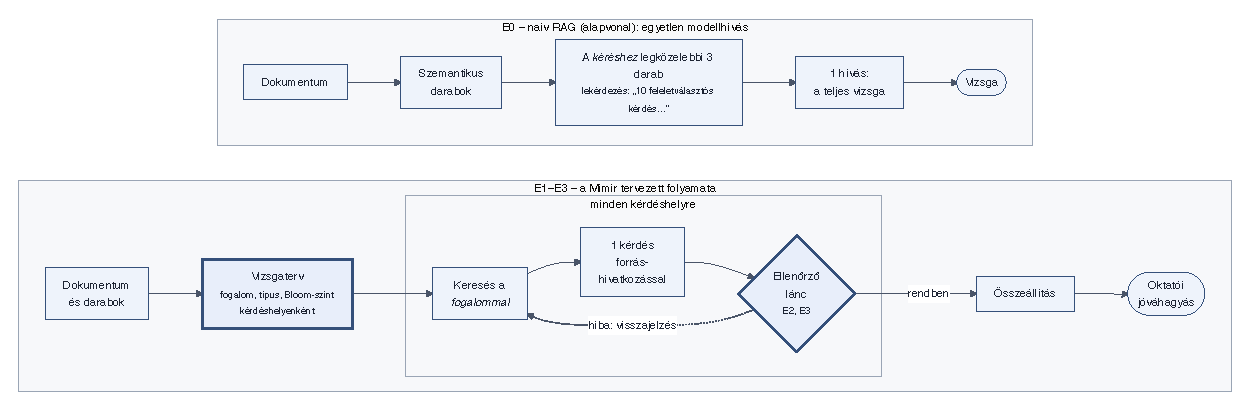
\includegraphics[width=\textwidth]{figures/d2_folyamatok}
\caption[A naiv RAG és a \Mimir{} tervezett generálási folyamata.]{A naiv RAG és a \Mimir{} tervezett generálási folyamata. A terv a vizsga szerkezetét még az
első kérdés megírása előtt rögzíti, és minden kérdést a saját, hivatkozott kontextusával szemben
ellenőriz.}
\label{fig:pipelines}
\end{figure}

A módszer modellfüggetlen: minden nyelvimodell-hívás OpenAI-kompatibilis felületen megy át, a generátor
egy konfigurációs kulccsal cserélhető. A vizsgálatokban a Qwen2.5-7B~\cite{qwen25} (pilot és előzetes
vizsgálat), valamint a NYTK magyarra továbbtanított, Llama-3.1 alapú PULI-LlumiX 8B~\cite{pulillumix} és
a Gemma 3 12B~\cite{gemma3} (fő vizsgálat) volt a generátor. Mindhárom 4 bites (Q4\_K\_M, kb.\ 4,8
bit/súly) kvantálással fut az Ollamán~\cite{ollama2024}, $T=0{,}2$ hőmérséklettel és 8\,192 tokenes
kontextussal (a \arm{B-doc-L} 16\,384 tokennel); a fő vizsgálatban a válasz legfeljebb 4\,096 token
(\code{num\_predict}). A kísérleti \arm{E0} az éles útvonal promptját használja, de ezekkel a
paraméterekkel, a keretrendszerben; az éles végponton át futó kontrollkonfiguráció nem futott
(\ref{sec:karok}.~szakasz).

% ---------------------------------------------------------------------
\subsection{Szemantikus darabolás}
\label{sec:darabolas}
% ---------------------------------------------------------------------

A RuneCarver a szöveget mondatokra bontja, minden mondathoz 768 dimenziós vektort rendel a
multilingual-E5-base~\cite{wang2024me5} kódolóval (a mondat tokenjei vektorainak átlagát, hosszabb
szövegablakban, így a szomszédos mondatok jelentése is benne van), és ott vág, ahol két szomszédos mondat
koszinusz-távolsága meghaladja a vágási küszöböt: alapértelmezésben a távolságok 85.~percentilisét,
vagyis a legnagyobb 15\,\% távolságnál. A célméret (1\,000 karakter) túllépése után a küszöb arányosan
csökken; ez a \emph{puha korlát} mondat közepén soha nem vág (a képlet: \ref{app-darabolas}.~függelék).
A szemantikus darabolás az éles rendszerben és a kiértékelésben ugyanaz a kód; csak a rögzített
darabolású \arm{E5c} darabol a keretrendszerben.

\paragraph{A csonkolt kódoló hibája.}\label{sec:csonkolt} A kódoló legfeljebb 512 tokenes bemenetet fogad.
Az eredeti implementáció a teljes dokumentumot egy menetben, csonkolva kódolta, így az 512.~token után
kezdődő mondatok nullvektort kaptak, és hosszabb dokumentumon a vágás már nem a tartalomtól, csak a darab
hosszától függött. A javított kódoló mondathatáron vágott, legfeljebb 510 tokenes ablakokban dolgozik
(rövid szövegen az eredmény azonos). Az \arm{E5a} a régi kódolót szándékosan megtartja, hogy a hiba
hatása mérhető legyen.

% ---------------------------------------------------------------------
\subsection{Indexelés és az alapvonalak}
% ---------------------------------------------------------------------

A darabokat a Bifrost az E5 kódolóval beágyazza, és a Qdrant-vektortárba tölti, amely minden új
dokumentum előtt kiürül; a \emph{sűrű keresés} a lekérdezéshez koszinusz-hasonlóság szerint legközelebbi
$k$ darabot adja vissza. Az \arm{E0} lekérdezése a felhasználói kérés szövege („Készíts pontosan 10 darab
vizsgakérdést, típus: feleletválasztós\ldots”), kontextusa a három leghasonlóbb darab, promptja a rendszer
éles, v1.0-s promptja (\ref{app-prompt}.~függelék). A \emph{teljes dokumentumos prompt} (\arm{B-doc-L}
helyben, \arm{B-doc-S} a szerveren) ugyanezt a promptot használja a teljes dokumentummal (helyben
legfeljebb 30\,000, a szerveren 80\,000 karakter; a levágott rész arányát rögzítjük).

% ---------------------------------------------------------------------
\subsection{A vizsgaterv}
\label{sec:blueprint}
% ---------------------------------------------------------------------

\paragraph{Fogalomtervezés.} A tervező egyetlen hívásban a dokumentum \emph{áttekintését} kapja: minden
darab azonosítóját ($C_0, C_1,\dots$) és elejét, összesen legfeljebb 12\,000 karakterben (darabonként
legalább 120 karaktert). A modell így folytonos szöveg helyett azonosítókkal tagolt felsorolást lát, ami a
„lost in the middle” jelenség~\cite{liu2024lost} ellen hat. A tervező $n+3$ fogalmat ad vissza ($n$ a
kért kérdésszám), mindegyikhez egy mondatos leírást (mit kell kérdezni), az alátámasztó darabok
azonosítóit és egy fontossági értéket (1: részlet, 2: fontos, 3: központi). Értelmezhetetlen válasznál
darabonként egy álfogalom lép a helyükre, így a terv mindig létrejön.

\paragraph{Bloom-szintek és fogalomválasztás.} A kért nehézséghez egy Bloom-szint-eloszlás
tartozik~\cite{anderson2001bloom}, amelyet a legnagyobb maradék módszerével~\cite{balinski2001fair}
alakítunk egész darabszámokká (\ref{tab:bloom}.~táblázat, \ref{app-bloom}.~függelék). Az összeg mindig
pontosan $n$, így a nehézség nem kérés a promptban, hanem a terv szerkezeti tulajdonsága. A
kérdéshelyekhez egy \emph{mohó} eljárás választ fogalmat: mindig azt, amely még le nem fedett darabot
érint, ezen belül a legfontosabbat; ha minden darab le van fedve, a fontosság dönt. Ha a tervező legalább
$n$ fogalmat javasolt, a kérdések így nem tömörülhetnek a dokumentum egyetlen részére; kevesebb fogalomnál
a fogalmakat más Bloom-szinttel újra felhasználjuk, a ki nem választottak alkotják a
\emph{tartaléklistát}.

% ---------------------------------------------------------------------
\subsection{Kérdéshelyenkénti keresés}
\label{sec:visszakereses}
% ---------------------------------------------------------------------

Minden kérdéshely saját kontextust kap: a lekérdezés a fogalom neve és leírása, a kontextus a fogalomhoz
a tervező által rendelt első két darab, kiegészítve a keresés $k=3$ találatával (ismétlés nélkül),
legfeljebb 6\,000 karakterig. A lényegi különbség a naiv RAG-hoz képest, hogy a lekérdezés itt tartalmi
fogalom („immunológiai memória: hogyan alakul ki”), nem feladatleírás („10 kérdés, könnyű”). A
\emph{hibrid} változat (\arm{E2h}) a sűrű rangsort egy előtagtövesített BM25-rangsorral egyesíti reciprok
rangfúzióval (\ref{eq:rrf}.~egyenlet, \ref{app-hibrid}.~függelék).

% ---------------------------------------------------------------------
\subsection{Forráshoz kötött kérdésgenerálás}
\label{sec:generalas}
% ---------------------------------------------------------------------

A generátor egyetlen kérdést ír a kérdéshely terve szerint. A prompt (\ref{app-prompt}.~függelék)
megadja a fogalmat, a kérdezendő tartalmat, a típusszabályt (négy válasz, egy helyes), a Bloom-szint
magyar leírását, a nehézséget és a nyelvet; megismétli az éles prompt szabályait; felsorolja a már
elfogadott kérdéseket; és megköveteli a \code{citations} mezőt, amelyben a modell megnevezi a kulcsot
igazoló darabok azonosítóit. Így minden kérdés saját, ellenőrizhető forrásrészlethez kötődik (G1).

% ---------------------------------------------------------------------
\subsection{Az ellenőrző lánc}
\label{sec:verifier}
% ---------------------------------------------------------------------

Az ellenőrzések a legolcsóbbtól a legdrágábbig futnak (\ref{tab:checks}.~táblázat;
a visszacsatolás folyamatábrája: \ref{fig:ellenorzo}.~ábra, \ref{app-slot}.~függelék): ha egy szabályalapú ellenőrzés hibát talál, a nyelvi modellt igénylő
ellenőrzések el sem indulnak. A modellalapú ellenőrzések forrása a kérdés által hivatkozott darabok. A
lánc a kiértékelő keretrendszer része, nem azonos a Heimdall mai, egyetlen pontszámot adó lépésével.

\begin{table}[htbp]
\centering
\caption{Az ellenőrző lánc lépései végrehajtási sorrendben, a hiba esetén adott visszajelzéssel.}
\label{tab:checks}
\small
\begin{tabularx}{\textwidth}{@{}>{\raggedright\arraybackslash}p{3.8cm}c>{\raggedright\arraybackslash}X@{}}
\toprule
Ellenőrzés & LLM-hívás & Visszajelzés hiba esetén \\
\midrule
Forma & -- & feleletválasztós kérdés: 4 válasz, ebből 1 helyes \\
Meta-hivatkozás & -- & fogalmazd meg „a szöveg szerint” jellegű hivatkozás nélkül \\
Szivárgás és kérdésforma \emph{(a pilot után)} & -- & a törzs ne tartalmazza a választ, és legyen valódi kérdés \\
Hivatkozás & -- & hivatkozz a kontextus legalább egy darabjára \\
Alátámasztottság és disztraktorok & 1 & a kulcsot a részlet nem igazolja / egy disztraktor igaz lehet / kétértelmű \\
Vak megoldás & 1 & egy független megoldó más választ jelölt meg \\
Duplikátum & -- & túl hasonló egy már elfogadott kérdéshez \\
\bottomrule
\end{tabularx}
\end{table}

A \emph{szivárgási szabály} akkor jelez, ha a legalább háromszavas kulcs szavainak legalább 80\,\%-a a
törzsben (a kérdés szövegében) is szerepel, a \emph{kérdésforma-szabály} akkor, ha a törzs sem kérdőjelre,
sem kettőspontra nem végződik; mindkettőt a pilot hibamódja (\ref{sec:szivargas}.~szakasz) motiválta.
Az \emph{alátámasztottsági} hívás azt kérdezi, igazolja-e a forrás a kulcsot, hamis-e minden disztraktor
és kétértelmű-e a kérdés; a \emph{vak megoldásban} a modell a kulcs ismerete nélkül, összekevert
válaszokkal dönt. \emph{Duplikátum} a legalább 0,9 koszinusz-hasonlóságú kérdés. Az ellenőrzést maga a
generátor végzi, az \arm{E2x}-ben egy másik modell (Llama-3.1-8B~\cite{grattafiori2024llama3}).

A hibák listája visszajelzésként a következő kísérlet promptjába kerül ($r=1$ újrapróbálkozás, majd egy
tartalékfogalom); ha a kulcs nem igazolt, a keresés két darabbal bővül. Ha így sem sikerül, a legjobb
kísérlet \emph{nem ellenőrzöttként} megjelölve marad meg, hogy az oktató lássa; hibás formánál egy
\emph{javító} hívás pótolja a hiányzó disztraktorokat (\ref{alg:slot}.~algoritmus,
\ref{app-slot}.~függelék). Az \arm{E1} csak a formát, a meta-hivatkozást és a duplikátumot vizsgálja. A
technikai hiba miatt elmaradt ellenőrzés a kérdést nem tartja fel, de naplózzuk.

\paragraph{Költség.} Az egyhívásos konfigurációk (\arm{E0}, \arm{E5a}--\arm{E5c}, \arm{B-doc}) egy
hívással dolgoznak, az \arm{E1} legalább $1+n$ (tervezés és kérdésenként egy generálás), az \arm{E2}
legalább $1+3n$ hívással (kérdésenként generálás, alátámasztottsági ellenőrzés és vak megoldás). Tíz
kérdésnél ez 11, illetve 31 hívás, ha minden kérdés elsőre átmegy; minden elutasítás további két-három
hívással jár.

% ---------------------------------------------------------------------
\subsection{Munkamenet-hatókörű fogalomgráf}
\label{sec:graf}
% ---------------------------------------------------------------------

Az \arm{E3} a tervezőhívást egy fogalomgráffal váltja ki: kötegenként kinyeri a fogalmakat, a rövid
tényeket és a fogalmak közötti kapcsolatokat, a fogalmakat centralitás szerint rendezi, és ez a lista lép
a tervező helyébe; disztraktor-ötletként a generátor a fogalom testvérfogalmait kapja
(\ref{app-graf}.~függelék). A gráf csak a vizsga élettartamáig létezik, a memóriában.

% ---------------------------------------------------------------------
\subsection{Összeállítás és emberi felügyelet}
\label{sec:felugyelet}
% ---------------------------------------------------------------------

Az elfogadott kérdéseket Bloom-szint szerint rendezzük, és mindegyikhez rögzítjük a hivatkozott
darabokat, a tervezett fogalmat és az \emph{ellenőrzött} jelzőt. A vázlat a webes szerkesztőbe kerül
(\ref{fig:szerkeszto}.~ábra), ahol az oktató szerkesztheti, átrendezheti és törölheti a kérdéseket,
módosíthatja a kulcsot, egyetlen kérdést újragenerálhat, és minden kérdés alatt látja a hivatkozott
forrásrészletet a fájl nevével és oldalszámával. Jóváhagyás nélkül semmi sem exportálható, az export
pedig feltünteti az MI-rendszer közreműködését és a modellt (G5). A szerkesztő a legacy és a v1 módban
ugyanaz, a jóváhagyás mindkettőben kötelező; a forrásrészlet azonban csak hivatkozást hordozó kérdésnél
jelenik meg, a mai naiv RAG-kimenetben ilyen nincs, ezért élesben az oktató ma forráshivatkozás nélkül
hagyja jóvá a kérdéseket.

\begin{figure}[htbp]
\centering
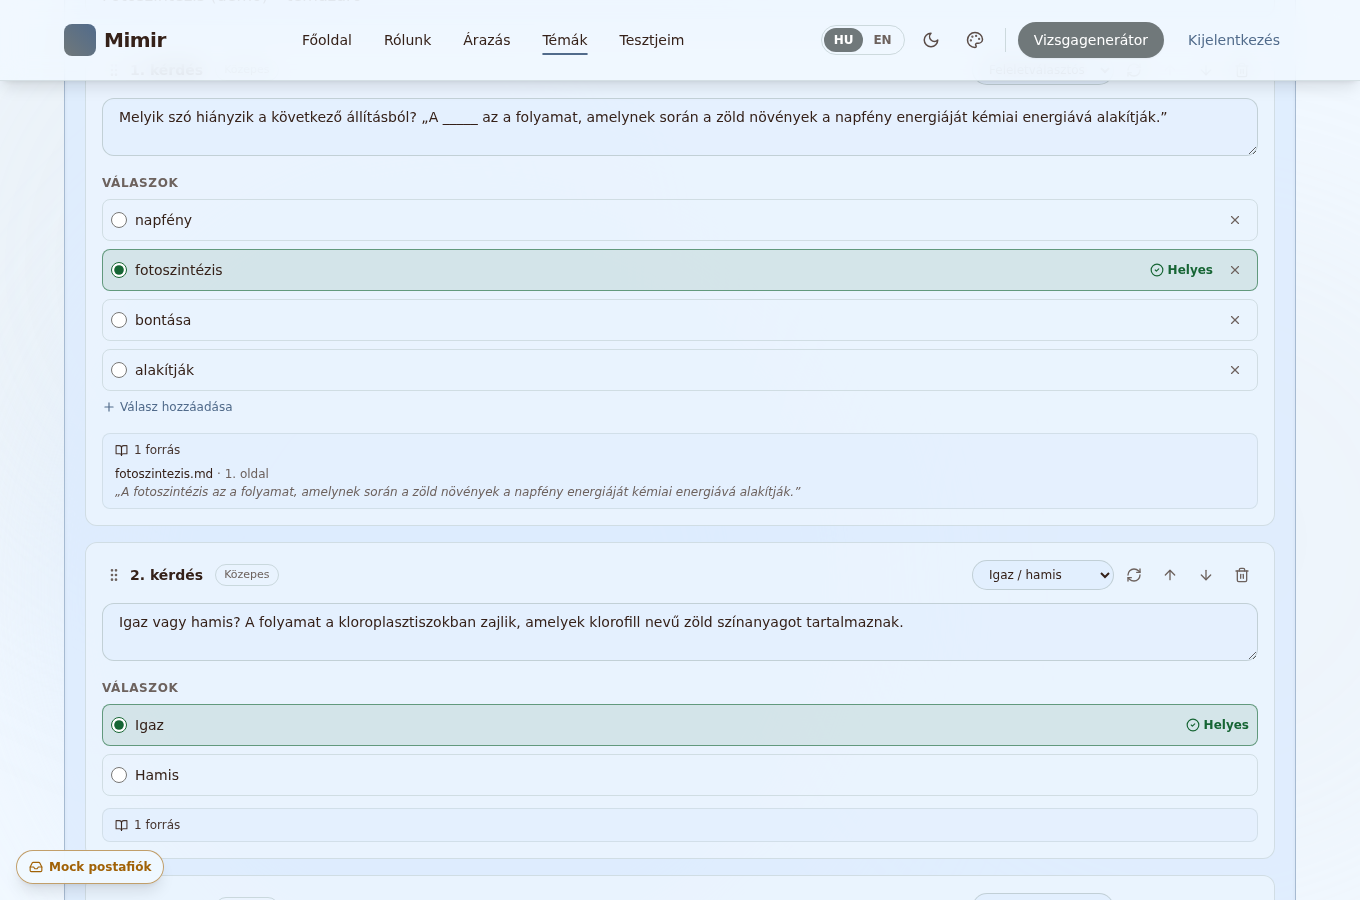
\includegraphics[width=0.75\textwidth]{figures/k1_szerkeszto.png}
\caption[A webes szerkesztő egy generált feleletválasztós kérdéssel.]{A webes szerkesztő egy generált
feleletválasztós kérdéssel: a megjelölt helyes válasz, alatta a hivatkozott forrásrészlet („1 forrás”,
fájlnév és oldalszám); jobb felül a típusválasztó, az újragenerálás, az áthelyezés és a törlés gombja. A
forrásrészlet a v1 API-szerződés kérdésenkénti hivatkozásából jelenik meg.}
\label{fig:szerkeszto}
\end{figure}

\bigskip
\noindent\textbf{A fejezet tanulsága.} A \Mimir{} mai változata adatvédelmi szempontból gondosan
kialakított naiv RAG-rendszer: a feldolgozási adatok a feladat végén törlődnek, az audit napló tartalmat
nem tárol, a helyi mód kapcsolható, az oktatói jóváhagyás kötelező. Az ellenőrizhetőség (G1) és a
kontrollált szerkezet (G2) a keretrendszerben elkészült módszerben van meg. Az élesítéshez el kell
dönteni, mely lépések érik meg a költségüket (\ref{ch:diszkusszio}.~fejezet), meg kell valósítani a v1
API-szerződést, valamint a hitelesítést és a témakörönkénti adatelkülönítést, amelyek nélkül a rendszer
többfelhasználós üzemre nem alkalmas.
